\documentclass[a4paper, 12pt]{article}

% Layout
\usepackage{geometry}
\geometry{left=16mm}
\geometry{right=10mm}
\geometry{top=1cm}
\geometry{bottom=1cm}

% Paragraph
\usepackage{indentfirst}
\setlength{\parindent}{0.75cm}
\linespread{1.25}

% Font
\usepackage{fontspec}
\usepackage[english,russian]{babel}
\usepackage{microtype}

% \usepackage{polyglossia}
% \setmainlanguage{russian}
% \setotherlanguage{english}

% \newfontfamily{\cyrillicfont}{Droid Serif}
% \newfontfamily{\cyrillicfontrm}{Droid Serif}
% \newfontfamily{\cyrillicfontsf}{Droid Sans}
% \newfontfamily{\cyrillicfonttt}{DejaVu Sans Mono}

\setmainfont{Times New Roman}
\setromanfont{Times New Roman}
\setsansfont{Droid Sans}
\setmonofont{DejaVu Sans Mono}

% Hyphens
\usepackage{hyphenat}
\usepackage{ucharclasses}
\setTransitionsForLatin{\begingroup\hyphenrules{english}}{\endgroup}

% Formulas
\usepackage{amssymb, amsfonts, amsmath}

% Miscellaneous
\usepackage{enumerate}
\usepackage{float}
\usepackage{multirow}

% Hyper references
\usepackage{hyperref}
\hypersetup{
    hidelinks,
    allcolors=black
}

% Images
\usepackage{graphicx}
\graphicspath{ {images/} }

%Including title
\usepackage{pdfpages}

% Figures
\usepackage{chngcntr}
\counterwithin{figure}{section}
\usepackage{subcaption}
\renewcommand\thesubfigure{\asbuk{subfigure})}
\captionsetup[subfigure]{labelformat=simple, labelsep=space}

% Counters
\usepackage[figure,table,page]{totalcount}
\usepackage{totcount}

% Code listings
\usepackage{listings}
\usepackage{xcolor}

\definecolor{codegreen}{rgb}{0,0.6,0}
\definecolor{codepurple}{rgb}{0.58,0,0.82}
\lstdefinestyle{codestyle}{
    commentstyle=\color{codegreen},
    keywordstyle=\color{magenta},
    stringstyle=\color{codepurple},
    basicstyle=\ttfamily\footnotesize,
    breakatwhitespace=false,
    breaklines=true,
    captionpos=b,
    keepspaces=true,
    showspaces=false,
    showstringspaces=false,
    showtabs=false,
    tabsize=2
}

\bibliographystyle{gost780s}



\newtotcounter{citenum} %From the package documentation
\def\oldbibitem{}
\let\oldbibitem=\bibitem
\def\bibitem{\stepcounter{citenum}\oldbibitem}

\begin{document}
\includepdf[pages={1}]
{title.pdf}

\tableofcontents
\newpage

\section{Введение}
Обеспечение кибербезопасности на сегодняшний день является одной из наиболее актуальных проблем.
Она давно поднялась с уровня частных лиц до уровня крупных организаций. Возникла необходимость
создания интеллектуальных систем (ИС), способных автоматизировать процесс анализа степени защищенности
программного обеспечения этих организаций. Применение интеллектуальных систем в защите
информационного пространства охватывает очень широкий круг направлений.
В настоящий момент такие системы используются в следующих сферах \cite{spheres}:

\begin{itemize}
\item
Обеспечение информационной безопасности энергетических обьектов
\item
Обеспечение кибербезопасности бизнес-среды.
\item
Системы обнаружения,
предупреждения, реагирования на инциденты и ликвидацию последствий компьютерных атак.
\item
Интеллектуальные системы антивирусной защиты, применяются для контроля каналов проникновения вирусов,
для защиты от вирусов, ``червей'', нежелательных программ, для оповещения при ``заражении'', для ``лечения''
от вирусов.
\end{itemize}

Вторые так же могут служить основанием для когнитивных подходов к оценке кибербезопасности \cite{kognmodels}.

Некоторые из проектов интеллектуальных систем по обеспечению компьютерной безопасности
на данный момент существуют только в концептуальном виде \cite{concept}, но есть и реализованные,
основанные на онтологиях или технологии интеллектуальных многоагентных систем \cite{multigent}.

Цель данной работы --- рассмотреть применение интеллектуальных систем для обеспечения компьютерной
безопасности различных общественных структур и изучить самые популярные подходы
к построению такого рода систем.

\newpage
\section{Борьба с киберугрозами в энергетической сфере}
Одна из сфер, где наиболее востребованы интеллектуальные системы для поиска информационных угроз
является отрасль энергетики. Цифровизация ее объектов может вызвать возникновение киберугроз,
связанных с внедрением новых решений, применением новых безнес-моделей, сопровождающихся отсутствием
или недостаточностью информации для оперативного принятия решений по обеспечению безопасности объекта.
Требования, предъявляемые к таким системам описаны в работе \cite{reqs}.

Построение ИС, ответственной за данную задачу, происходит по схеме, представленной
в работах \cite{scheme, ontoling}.
Общая структура такой системы включает три компонента:
\begin{itemize}
\item
Экспертную систему (ЭС) ``Cyber'' -- продукционная ЭС, предназначенную для выявления типовых уязвимостей,
угроз и векторов атак ИТС объекта;
\item
Блок байесовских сетей доверия, ответственный за моделирование экстремальных ситуаций, вызванных нарушением
кибербезопасности, определения вероятности наступления последствий;
\item
Блок оценки рисков наступления экстремальной ситуации и последствий от реализации киберугроз
\end{itemize}

\subsection{Экспертная система ``Cyber''}
В работе \cite{cyber} архитектура экспертной системы ``Cyber'' рассмотрена более подробно.
Разработка интеллектуальной системы основана на методике анализа угроз и оценки рисков нарушения
информационной безопасности энергетических комплексов \cite{methods}.
Экспертную систему было решено проектировать с использованием продукционной модели знаний,
которая позволяет отобразить экспертные данные в базе знаний в виде правил ЕСЛИ – ТО. ЭС
включает три структурных элемента:
\begin{itemize}
\item Графический интерфейс пользователя;
\item Интерфейс взаимодействия;
\item Ядро экспертной системы.
\end{itemize}

База знаний представляет собой совокупность шаблонов (DEFTEMPLATES) и правил (RULES), а
также вспомогательных функций (FUNCTION), обеспечивающих организацию фактов в базе знаний.
В системе заложены три группы правил:
\begin{itemize}
    \item Правила определения угроз по выбранному ответу пользователя с отметкой уязвимости;
    \item Правила вывода мер защиты ресурса от выявленных угроз для каждой уязвимости в
    зависимости от класса защищенности автоматизированной системы управления (АСУ);
    \item Общие правила вывода мер защиты ресурса от выявленных угроз для каждой уязвимости.
\end{itemize}

Внутренний алгоритм работы  ЭС ``Cyber'' состоит в следующем: система содержит ряд вопросов
по безопасности автоматизированной системы управления предприятием с вариантами ответов.
Ввод условий осуществляется посредством опрашивания пользователей с предложением вариантов ответов.
Получив ответы пользователя, система вносит факты о наличии уязвимостей и угроз, связанных с
реализацией выявленных уязвимостей, в базу знаний.

Угрозы с высокой степенью представляют наибольший риск нарушения безопасности для предприятия.
Факты, соответствующие низкой и средней степени угроз, удаляются из базы знаний. Для высокой
степени угроз системой формируется набор мер по обеспечению безопасности и выводится на экран.

До начала основного опроса пользователю предлагается выбрать уровень защищенности АСУ, который
влияет на критичность уязвимостей угроз и выбор меры обеспечения безопасности.

\subsection{Интегрированные байесовские сети доверия}
Байесовские сети доверия (БСД) отвечают за построение сценариев вероятных угроз. Для БСД
разработана онтология сценария экстремальной ситуации в энергетике, вызванной нарушением
кибербезопасности на объекте. Такой сценарий представляет собой вероятностные оценки возможных
ситуаций, представленные последовательностью уязвимостей, киберугроз, угрозами причинения ущерба
предприятию либо энергосистеме в целом. В процессе формирования графа экстремальной ситуации
оценивается вероятность наступления некоторых негативных событий. В работе по исследованию
энергетической безопасности \cite{secur} разработаны опознавательные признаки, по которым система судит о наступлении
той или иной ситуации.

\subsection{Оценка рисков}
Анализ рисков проводится в рамках решения задач по анализу киберугроз и моделированию сценариев
экстремальных ситуаций в энергетике. После онтологического инжениринга система оценки рисков будет состоять
из следующих компонент:
\begin{itemize}
\item
Идентификация рисков (осуществляется при анализе угроз, поддерживаемой онтологией оценки рисков)
\item
Анализ риска (осуществляется при моделировании сценариев, поддерживаемого онтологией оценки рисков)
\item
Оценивание рисков (поддерживается онтологией критериев ранжирования, онтологией рисков кибербезопасности,
онтологией рисков и критериев оценки)
\end{itemize}
В данном контексте риск рассматривается как сочетание последствий некоторого инцидента и связанной с ним возможностью
возникновения. Оценка рисков --- процесс идентификации, анализа и оценивания, в соответствии со стандартом
ISO/IEC 27005:2011.

На заключительном этапе оценки рисков предполагается проводить ранжирование объектов. Для этого вводится
критерий значимости объекта, зависящий от критерия оценки рисков, интегрального показателя рисков объекта,
объекта, представленного совокупностью основных характеристик.
\subsection{Работа всех трех ключевых компонент как единого целого}
Основные задачи, которые решает интеллектуальная система: анализ киберугроз, моделирование сценариев,
и оценивание рисков. Для ее реализации была придумана совокупность систем онтологий, отвечающих за
отдельные аспекты проблемы. Схема этой системы представлена на рис. \ref{dio}.

\begin{figure}[h]
    \center{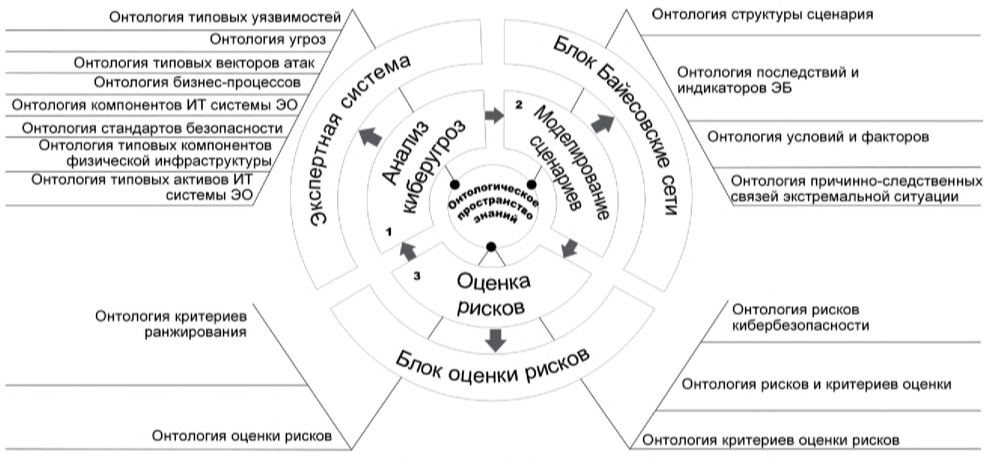
\includegraphics[width=1\linewidth]{scheme}}
    \caption{Строение системы онтологий}
    \label{dio}
\end{figure}

Из данной схемы ясно, что для каждой из основных предметных областей создается набор онтологий, связанных
между собой. В разделе, связанным с анализом киберугроз, онтологический инжениринг позволяет систематизировать
информацию об различных информационно-технологических характеристиках конкретных энергетических объектов
и создать базу знаний их уязвимостей и угроз.

\textbf{Онтология стандартов безопасности} разрабатывается с целью кластеризации знаний по методам проведения оценки
безопасности. Впоследствии она послужит компонентом для проведения
аудита безопасности предприятий, проводимого с использованием ``Cyber'' и моделировании сценариев возможных
экстремальных ситуаций.

За определение основных угроз в системе антологий, предлагаемой в работе \cite{ontoling}, отвечает \textbf{
онтология угроз}. Ключевая задача этой онтологии --- установление самых актуальных уязвимостей в энергетике.

После полного цикла работы данной интеллектуальной системы пользователь получает список объектов энергетики,
упорядоченный по степени уязвимости к кибератакам или иным экстремальным ситуациям в области кибербезопасности.

\newpage
\section{Интеллектуальные системы в кибербезопасности телекоммуникаций}
Большинство современных систем кибербезопасности (КБ) телекоммуникационных сетей и технологий (ТКСиТ)
являются сложными управляемыми системами \cite{tels},
разработка которых требует постоянного анализа тенденций их развития, направлений совершенствования
технологий их построения. В отличие от
процесса разработки системы кибербезопасности ТКСиТ, реализация которого требует принятия технических решений по всему перечню
решаемых задач проектирования различными специалистами (группами специалистов), процесс экспертной
деятельности должен быть направлен на формирование экспертных оценок, основанных на анализе некоторых
обобщенных показателей качества проектируемой системы, характеризующих стратегические технические
решения (технические решения, определяющие облик системы кибербезопасности в целом) и осуществляется
сравнительно небольшой группой специалистов.

Суть подхода заключается в формировании экспертных показателей качества (ЭПК), отражающих уровень
КБ и существенные свойства СКБ ТКСиТ, формировании оптимальных (не избыточных) экспертных систем
показателей качества (ЭСПК), соответствующих физическому, канальному и сетевому уровню
кибербезопасности ТКСиТ, на основе моделей и алгоритмов, соответствующих характеру и степени априорной
неопределенности того или иного этапа функционирования данной системы. Очевидно, что реализовать
предложенные модели и методы в ходе организации экспертной деятельности в интересах анализа
кибербезопасности ТКСиТ возможно только на основе разработки специальных экспертных систем.

Основу знаний, содержащихся в специальной ЭС должны составлять знания:
содержащиеся в памяти эксперта-донора; полученные в результате моделирования процессов изменения ЭПК КБ
ТКСиТ; полученные в результате анализа данных, поступающих из системы-аналога; содержащиеся на
материальных носителях (компакт диски, специальная литература и т.д.). В настоящее время разработаны
десятки моделей (языков) представления знаний для различных предметных областей. Все многообразие моделей
можно разбить на две большие группы – модульные и сетевые. Поскольку модульные модели оперируют
совокупностью не связанных элементов знаний и предназначены для интерпретации только поверхностных
знаний в специальной ЭС такого класса должны быть реализованы сетевые языки представления знаний.

\newpage
\section{Интеллектуальные системы и кибербезопасность в бизнес-среде}
Третьей, но оттого не менее важной областью применения ИС для обеспечения информационной безопасности
является бизнес-среда. В данном случае многоагентный подход находит широкое применение в
областях, требующих решения сложных задач: реинжиниринг бизнес-процессов,
построение виртуальных предприятий, имитационное моделирование интегрированных производственных систем
и т.д \cite{mob}. Наибольшую сложность в теоретических исследованиях и практических реализациях современных
многоагентных систем представляют вопросы, связанные с обеспечением информационной безопасности агентов и информационных
ресурсов, которыми они оперируют, в открытых многоагентных виртуальных средах.

В качестве примера автор работы \cite{mob} приводит решение задачи
обеспечения информационной безопасности в объектах многоагентной
системы информационной поддержки инноваций, реализующей
открытую многоагентную виртуальную бизнес-среду инновационной деятельности.

С точки зрения общей логики функционирования такая среда имеет многоагентную реализацию.
Агентная ориентированность выражается в том, что в ней каждый субъект инновационной деятельности
представлен одним или несколькими мобильными агентами, которые представляют предложения
своих владельцев и реализуют процедуры автоматизированного поиска партнеров для сотрудничества.

В общем случае такая многоагентная система, какая описана в работе \cite{mob}, задается отношением множеств
пользователей системы, ее агентов, представляющих их интересы в бизнес-среде, множества узлов системы,
множества виртуальных бизнес-площадок, множества информационных ресурсов системы, множества атрибутов объектов модели.
Два основных типа агентов системы: мобильные агенты и управляющие агенты. Первые перемещаются между узлами сети,
а вторые координируют процессы взаимодействия и миграции первых.

Для решения задачи обеспечения кибербезопасности в распределенной многоагентной системе авторами статьи \cite{mob}
предлагается метод формирования комплексной самоорганизующейся системы децентрализованного управления безопасностью
мобильных агентов, аутентификация мобильных агентов в которой осуществляется через открытые ключи и
удостоверяющие их центры.

В предлагаемой системе формирование удостоверяющих центров будет осуществляться автоматически на основе механизмов
самоорганизации агентов а функции управления процедурой выдачи сертификатов будут возложены на программных
управляющих агентов.

Самоорганизация заключается в автоматическом формировании виртуальных площадок, объединяющих
агентов с близкими целями в коалиции, и генерации управляющих агентов, выполняющих функции удостоверяющих центров
сертификации, для каждой площадки.

Система безопасности мобильных агентов может быть как централизованной, так и децентрализованной.
\begin{figure}
    \center{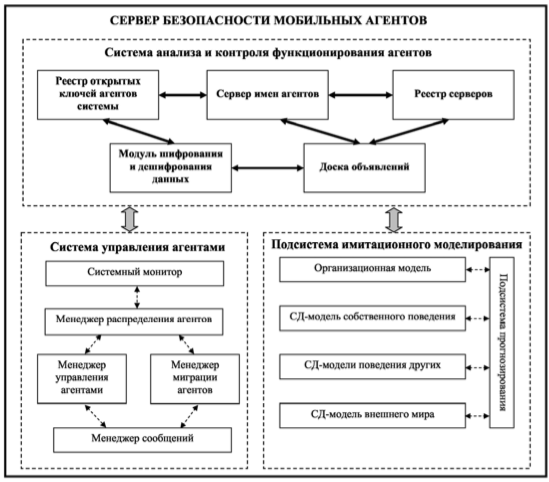
\includegraphics[width=13cm, height=10cm]{mobag}}
    \caption{Система безопасности мобильного агента(под централизованным управлением) \cite{mob}}
    \label{mobag}
\end{figure}

В случае использования системы с \textbf{централизованным} управлением безопасностью мобильных агентов в
открытой многоагентной виртуальной бизнес-среде, оно реализуется на выделенном сервере, функциональная
структура которого состоит в следующем: сервер безопасности мобильных агентов обеспечивает
централизованное хранение информации об агентах системы, доступных узлах, виртуальных бизнес-площадках,
открытых ключах агентов, доступ к которым имеют только управляющие агенты системы. Здесь же реализуются
модуль шифрования и дешифрования данных, а также система мониторинга, анализа и моделирования поведения
агентов системы, которая также доступна управляющим агентам системы.

В случае использования системы с \textbf{децентрализованным} подходом управление безопасностью мобильных агентов
в виртуальной бизнес-среде реализуется на каждом из серверных узлов системы
(порталов), на которых пользователи регистрируют свои предложения. При таком решении система безопасности
мобильных агентов является
частью агентного представительства серверного узла и выполняет аналогичные функции, что и сервер безопасности
мобильных агентов: хранит информацию об агентах системы, доступных узлах, виртуальных бизнес-площадках,
открытых ключах агентов, доступ к которым имеют только управляющие агенты системы, реализует процедуры
шифрования и дешифрования данных агентов, осуществляет мониторинг, анализ и моделирование поведения агентов
системы.

Централизованная система в сравнении с децентрализованной обладает рядом недостатков \cite{probs}: % Проверить что цитата по теме
\begin{enumerate}
    \item уязвимость центрального звена (при отказе сервера безопасности
    нарушается защита активных компонентов и всей системы в целом, ее безопасность становится под угрозой);
    \item высокая нагрузка на центральный сервер управления безопасностью при большом количестве агентов
    и узлов и, как следствие – ограниченная масштабируемость;
    \item централизованное администрирование подразумевает полный контроль над ресурсами на стороне сервера,
    что не всегда приемлемо, если ресурсы принадлежат разным пользователям
\end{enumerate}

Помимо описанных выше минусов, согласно работе \cite{mob}, централизованное управление безопасностью
гораздо менее продуктивно и намного более длительно чем децентрализованное. При увеличении количества
узлов и мобильных агентов увеличивается нагрузка на центральный
сервер безопасности мобильных агентов, тем самым уменьшается производительность МАС.

Ввиду описанных выше аспектов, использование децентрализованной системы для обеспечения
безопасности мобильных агентов предпочтительно.

\newpage
\section{Другие идеи для применения интеллектуальных систем в кибербезопасности}
Интеллектуальные системы применяются в контексте кибербезопасности не только в тех областях, о которых было
написано выше. Существуют и не совсем обычные проекты, связанные с этой отраслью.

\subsection{Концепция интеллектуальной системы обеспечения кибербезопасности сверхзвукового
пассажирского самолета}
Конструктивное решение по обеспечению информационной безопасности воздушного средства (ВС), должно гарантировать
невозможность перехвата управления и нарушение работоспособности оборудования и систем ВС (
Это решение так же должно реализовывать такие требования безопасности как контроль и управление доступом,
обеспечение целостности ресурсов, обеспечение защиты конфиденциальности при хранении и передачи информации
и др.
) \cite{concept}. Так же система обеспечения кибербезопасности должна иметь возможность функционировать в
условиях реального времени и использовать современных технологий сотовой, спутниковой и
радиосвязи для передачи больших объемов данных.
Для предотвращения потенциальных киберинцидентов необходимо использовать комплексный подход
к управлению киберрисками ВС. Данный подход должен включать в себя последовательный ряд процедурных
и технических решений по предотвращению киберинцидентов и последствий от них.
Он будет состоять из следующих этапов:

\begin{enumerate}
\item
Выявление угроз (внутренних и внешних)
\item
Идентификация уязвимостей (Определение перечня бортового оборудования, имеющего проводные / беспроводные каналы
информационного взаимодействия. Прогноз возможных последствий угроз кибербезопасности каждой системы.
Определение возможностей и ограничений применения на борту ВС существующих способов защиты.)
\item
Оценка подверженности рискам (Определение вероятности уязвимости от внешних / внутренних угроз,
ошибки при создании и закладки ПО, преднамеренное /
непреднамеренное негативное влияние
человека при эксплуатации оборудования)
\item
Разработка способов обнаружения и защиты (Снижение вероятности уязвимости через защитные меры. Уменьшение
потенциального воздействия уязвимостей при эксплуатации)
\item
Локализация отказа и сохранение безопасной эксплуатации (Разработка алгоритма локализации последствий
киберинцидента, реконфигурация оборудования для сохранения безопасной эксплуатации ВС, сниение любого потенциала
выявленных киберрисков.)
\item
Очистка и восстановление после киберинцидента (Разработка алгоритма действий по устранению последствий
киберинцидента и восстановлению системы.)
\end{enumerate}

Одной из перспективных систем организации воздушного движения, направленных
на интеграцию будущих систем связи, навигации, наблюдения и управления воздушным
движением (УВД), осуществляемую на базе общесистемного управления информации, является
система SWIM (System Wide Information Management) \cite{concept}. SWIM предназначена для обмена
данными и направлена на предоставление дополнительных услуг по управлению информацией
организации воздушного движения с использованием внешних сервисов ВС. Архитектура SWIM построена
на базе сервис-ориентированной архитектуры SOA (Service Oriented Architecture) \cite{soa}.

Программные комплексы, разработанные в соответствии с SOA, обычно реализуется как набор веб-служб,
взаимодействующих по протоколам SOAP, REST, XML. Основные преимущества использования веб-сервисов на основе SOA:
возможности расширения системы за счет модульности и автономности бизнес-серверов;
адаптивная настройка логики работы системы и изменение состава используемых компонентов без перекрытия;
повышение безопасности авиаперелетов за счет стандартизации процедур и протоколов для управления сетевой
и сервисной интеграции; безопасная интеграция с платформами и приложениями;
уменьшение стоимости и времени реализации проектов.

Архитектура SOA может быть реализована с использованием как сервисной, так и микросервисной архитектуры
приложений. Поддержка микросервисов позволяет использовать концепцию ``блокчейн как микросервис", и передачу
данных осуществлять в единой блокчейн инфраструктуре с открытым исходным кодом, которая устраняет недостатки
АЗН-В \cite{block} и обеспечивает высокий уровень доверия между участниками сервисного обмена.

Согласно \cite{concept}, внедрение блокчейн технологий увеличивает скорость обмена, уменьшает временные затраты, улучшает
качество, надежность и доступность услуг. При этом увеличивается прозрачность и надежность передачи
информации, снижаются киберриски.

Реализация предлагаемой концепции интеллектуальной системы обеспечения кибербезопасности бортового
оборудования и систем СПС, построенной на базе архитектуры SOA с использованием блокчейн технологий,
позволит сохранить работоспособность авиационных систем и оборудования, повысить безопасность полетов,
предотвратить человеческие жертвы и повысить степень комфорта пассажиров при возникновении киберугроз
на борту во время полета.
\subsection{Разработка экспертной системы для контроля информационной безопасности}
Работы \cite{scheme, ontoling} интегрировали в свои интеллектуальные системы экспертную систему ``Cyber''.
Но они не единственные, кто принял решение использовать экспертную систему в области безопасности информационного
пространства. В работе \cite{idea} автор, ориентируясь на различные банковские и бизнесс структуры, делает акцент на
доступности экспертной системы для пользователя. Поэтому он предлагает собственную архитектуру экспертной системы
(рис. \ref{arch}). Такая архитектура позволяет упростить работу с экспертной системой как со стороны пользователей,
так и со стороны ее проектировщиков.

\begin{figure}[h]
    \center{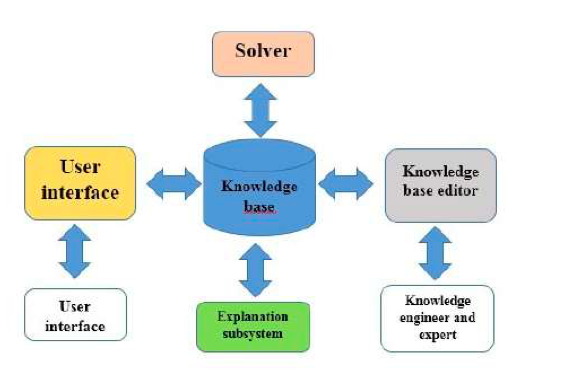
\includegraphics[width=11cm, height=6cm]{arch}}
    \caption{Архитектура экспертной системы \cite{idea}}
    \label{arch}
\end{figure}

Разработка данной экспертной системы состоит из нескольких этапов:
\begin{enumerate}
    \item
    Идентификация
    \item
    Концептуализация
    \item
    Формализация
    \item
    Реализация
    \item
    Тестирование
    \item
    Опытная эксплуатация
\end{enumerate}

На этапе \textbf{идентификации} определяются решаемые задачи, определяются цели разработки,
определяются эксперты и типы пользователей. Во время \textbf{концептуализации} проводится
содержательный анализ проблемной области, выявляются используемые понятия и их взаимосвязи,
определяются методы решения проблемы. После этого при \textbf{формализации}
выбираются и определяются способы представления всех видов знаний, формализуются основные
понятия, определяются способы интерпретации знаний, моделируется работа системы, способы
представления и манипуляции знаниями.

После этого наступает длительная ступень \textbf{реализации}. На этом этапе база знаний
заполняется экспертами и эта часть процесса самая важная и трудоемкая, поскольку происходит
упорядочение знаний, полученных от экспертов, что обеспечивает эффективную работу системы
в дальнейшем и представление знаний в виде ЭС. Реализация выполняется инженером по знаниям.
Стоит помнить, что начиная с этого этапа могут возникнуть определенного рода проблемы \cite{idea}.

Следующим шагом на пути к претворению в жизнь экспертной системы станут различного рода \textbf{тесты}.
На этом этапе выделяются ключевые проблемы проектируемой системы: какую информацию защищать, где она
расположена в базе знаний, какие устройства пользуются базой знаний, достаточно ли надежны пароли,
задаваемые пользователями и т. д... Для их решения задаются необходимые переменные и строятся логические
блоки с ветвлениями. После этого получается готовый продукт, достаточно удобный для потребителей.

\subsection{Применение онтологий в информационных войнах}
Понятие информационной войны подразумевает использование информационных и коммуникационных
технологий для достижения преимуществ по сравнению с потенциальным противником. В данном контексте
информационные структуры рассматриваются как системы, хранящие информацию, обрабатывающие ее и определяющие,
представляет тот или иной пакет угрозу или нет. Для этой цели используется онтологический подход к созданию
интеллектуальной системы, предоставляющей базу знаний для потенциального обучения на ней нейронной сети \cite{wars}
или иной самообучающейся системы.

Структура антологии, описанной в работе \cite{risk} базируется модели идентификации угроз STRIDE и методики DREAD
для оценки рисков угроз. В работе \cite{wars} она присутстсвует в упрощенном виде (см рис. \ref{ont}).

\begin{figure}[h]
    \center{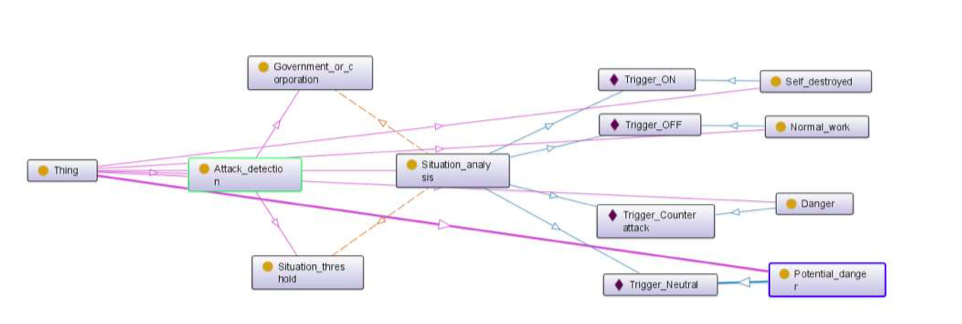
\includegraphics[width=1\linewidth]{ontology}}
    \caption{Структура онтологии для определения угроз \cite{wars}}
    \label{ont}
\end{figure}

В данной схеме Attack-detection есть абстрактный класс, включающий в себя ключевые аспекты предметной
области: Government or corporation (подкласс, определяющий к какому типу угроз относится поступающая угроза),
Situation analysis (подкласс, анализирующий ситуацию), различные тригеры, отражающие выводы к которым пришла
самообучающаяся система в результате анализа ситуации (``ON'' --- триггер немедленной остановки анализа и
признания атаки угрозой, ``OFF'' --- система воспринимает атаку как ложную и продолжает функционировать,
``NEUTRAL'' --- атака воспринимается как неизвестная потенциальная опасность, система продолжает функционировать,
но в отличие от ``OFF'' происходит более глубокий анализ атаки и причин ее возникновения с целью их
последующего устранения, ``“COUNTERATTACK'' --- атака расценивается как угроза, дальнейшие действия становятся
непредсказуемы)

Таким образом онтология, описанная выше, ложится в основу самообучающейся системы, способной идентифицировать
различные киберугрозы.

\subsection{Экспертные системы в кибербезопасности}
Существуют и проекты, посвященные оптимизации и ускорению процесса принятия решений. Учитывая постоянное
возрастание многообразия потенциальных и сложности реальных киберугроз, одним из вариантов
повышения эффективности принятия решений в области защиты
информации (ЗИ) и кибербезопасности стало внедрение разнообразных интеллектуальных
(или интеллектуализированных) программно-аппаратных комплексов в
данной области.

По мере усложнения сценариев кибератак стало очевидно \cite{opt}, что традиционные
сигнатурные методы не всегда в состоянии обеспечить должный уровень защиты
объектов информатизации.

Ключевая особенность подхода, который используется в проектируемой
АЭС (адаптивной экспертной системы), –-- применение ДПРПУ. Это позволило получать довольно высокие результаты в ходе тестовых экспериментов по распознаванию разновариантных угроз,
аномалий и кибератак.

Сравнивая с широко используемыми в системах выявления вторжений (кибератак) методами и моделями
(последовательный перебор признаков, статистические алгоритмы состояний),
модели, которые в своей основе содержали ДПРПУ, а
также разнообразные ОИО, дали значительный эффект. Так, в частности, сократился
объем необходимых правил для распознавания ОБР. Например, в рамках
класса сокращение правил составило 2,5–12 раз (зависит от класса ОБР – аномалия,
кибератака, киберугроза)

Следовательно, возможно добиться существенного снижения времени выяв-
ления аномалий, кибератак или угроз, а также последующей оценки их последствий
для ОБИ.
\newpage
\section{Заключение}
В заключении стоит сказать, что применение интеллектуальных систем в области компьютерной безопасности
достаточно широко. Были рассмотрены как уже созданные модели ИС, так и концепции, которые могут
быть реализованы в будущем. По итогам работы можно сделать вывод, что чаще всего ИС, ответственные за
кибербезопасность основаны на онтологиях, на многоагентных системах либо на экспертных системах.
Возможность использовать несколько компонентов сразу тоже вполне реальна.

Существуют и проекты, использующие либо оригинальные базы знаний и архитектуры, либо основанные на
готовых продуктах \cite{concept, wars}. Применяются они в банковской
сфере, в бизнесе, на энергетических объектах, а так же потенциально могут быть применены и в транспортной сети.

Но работа таких интеллектуальных систем далеко не всегда бывает быстрой и продуктивной \cite{mob, upg}. Это означает,
что следует и дальше развивать рассмотренные в данной работе технологии использования интеллектуальных
систем для обеспечения безопасности информационного пространства как крупных организаций и компаний, так
и частных лиц.
\newpage

\medskip
\begin{thebibliography}{}
\bibitem{spheres}
V. Tabakaeva, V. Selifanov, V. An, S. Bularga, and A. Vorozhtsov,
Intelligent information security management systems,  Trans. Sci. Pap. Novosib. State Tech. Univ., vol. 4,
no. 3–4, pp. 165–176., -2020
\bibitem{kognmodels}
Бурый А.С., Усцелемов В.Н. Онтологический подход к формированию когнитивных моделей оценки
кибербезопасности // Информационно-экономические аспекты стандартизации и технического
регулирования.,  No 3. (55). С. 77-84., -2020.
\bibitem{multigent}
И. В. Котенко, Интеллектуальные механизмы управления кибербезопасностью, -2009.
\bibitem{reqs}
Ворожцова Т. Н., Онтология как основа для разработки интеллектуальной системы обеспечения
кибербезопасности // Онтология проектирования., C.69-77., -2014
\bibitem{cyber}
А. Г. Массель, Д. А. Гаськова,Разработка экспертной системы для анализа угроз кибербезопасности в энергетических
системах // Information and mathematical technologies in science and management, No 1 (27), pp. 113-122, -2016
\bibitem{scheme}
D. Gaskova, A. Massel, The Technology of Cyber Threat Analysis and Risk Assessment of Cybersecurity
Violation of Critical Infrastructure // Vopr. kiberbezopasnosti, vol. 2, no. 2(30), pp. 42–49, -2019
\bibitem{ontoling}
А. Г. Массель, Д. А. Гаськова, Онтологический инжениринг для разработки интеллектуальной системы анализа угроз
и оценки рисков кибербезопасности энергетических объектов // Онтология проектирования, C. 255-238., -2019
\bibitem{methods}
А. Г. Массель, Методика анализа угроз и оценки риска нарушения информационно-технологической
безопасности энергетических комплексов // XX Байкальской Всероссийской конференции:труды,
т. III., С. 186-195., -2015.
\bibitem{secur}
Н И Пяткова, В И Рабчук, С М Сендеров, Энергетикая безопасность России: проблемы и пути решения / Новосибирск:
СО РАН, С. 198, -2011
\bibitem{tels}
Малофеев В. А., Паращук И. Б., Пронин А. А., Саяркин Л. А., Экспертные системы для анализа кибербезопасности
телекоммуникационных сетей и технологий, их задачи и особенности // ХVII САНКТ-ПЕТЕРБУРГСКАЯ
МЕЖДУНАРОДНАЯ КОНФЕРЕНЦИЯ, С. 114-115., -2020
\bibitem{mob}
А.В. Маслобоев, В.А. Путилов, Разработка и реализация механизмов управления информационной безопасностью
мобильных агентов в распределенных мультиагентных информационных системах // Вестник МГТУ, том 13, №4/2,
C. 1015-1032, -2010
\bibitem{probs}
А.В. Маслобоев, М.Г. Шишаев ,  Одноранговая распределенная мультиагентная система
информационноаналитической поддержки инновационной деятельности //
Научно-технический вестник СПбГУ ИТМО, № 4(62), C.108-114, -2009.
\bibitem{concept}
Зыбин Е.Ю., Кривоноженков В.А., Муллин А.Р., Кохан В.В., Концепция
интеллектуальной системы обеспечения кибербезопасности бортового оборудования
и систем сверхзвукового пассажирского самолета, ФГУП ``ГосНИИАС'', -2021
\bibitem{soa}
Z. Wang, X. Luo, M. Zhao and M. Qi,
The research of system wide information management based on SOA  // 6th
IEEE International Conference on Software Engineering and Service Science (ICSESS),
pp. 837-840., -2015
\bibitem{block}
Косьянчук В.В., Сельвесюк Н.И., Хамматов Р.Р. Обзор основных путей повышения безопасности системы АЗН-В
// Научный Вестник МГТУ ГА. 2019. Том 22, №01. С. 39-48.
\bibitem{idea}
T. Marzhan, Method of development of information security expert system, -2019, [Online].
Available: https://proc.ostis.net/wp-content/uploads/2019/10/OSTIS-2019.pdf
\bibitem{wars}
Научные Труды Конференции, “Open Semantic Technologies for Intelligent Systems”
// Inf.Tsu.Ru, vol. 7740, no. 3, pp. 145-150, -2019,
[Online]. Available: http://www.inf.tsu.ru/library/Publications/2020/2020-139.PDF.
\bibitem{risk}
P. Grabusts, O. Uzhga-Rebrov, Ontology-Based Risk Analysis System Concept.
// Open semantic technologies for intelligent systems, OSTIS-2017, Minsk, Belarus, pp. 341-346, -2017.
\bibitem{opt}
Ахметов Б.С., Лахно В.А., Досжанова А.А., Картбаев Т.С., Сабит Б. Модели для
адаптивной экспертной системы по выявлению киберугроз. // Проблемы информатики в
образовании, управлении, экономике и технике: Сб. статей XVIII Междунар. научно-техн. конф. Пенза:
ПДЗ, С. 84-90., 2018.
\bibitem{upg}
Коломойцев В.С., Богатырев В.А., Поляков В.И., Open Semantic Technologies for Intelligent Systems
// Inf.Tsu.Ru, vol. 7740, no. 3, pp. 315-320, -2019,
[Online]. Available: http://www.inf.tsu.ru/library/Publications/2020/2020-139.PDF.
\end{thebibliography}

\end{document}
